\documentclass[12pt]{report}

\usepackage{url}
\usepackage[margin=1.15in]{geometry}
\usepackage[T1]{fontenc}
\usepackage{lmodern} % monospace font
\usepackage[scale=0.89]{tgheros} % Helvetica is too big
%\usepackage[osf]{Baskervaldx} % tosf in text, tlf in math
%\usepackage[baskervaldx,cmintegrals,bigdelims,vvarbb]{newtxmath} % math italic letters from Baskervaldx
\usepackage[lf]{ebgaramond}
\usepackage{amsmath}
\usepackage[cmintegrals,cmbraces]{newtxmath}
\usepackage{listings}
%\usepackage{ebgaramond-maths}
\usepackage[cal=boondoxo]{mathalfa} % mathcal from STIX, unslanted a bit
\DeclareMathOperator{\Activ}{Activ}
\DeclareMathOperator{\Cost}{Cost}

\usepackage{setspace}

\lstset{basicstyle=\ttfamily, frame=single}
\usepackage{subcaption}
%\usepackage[draft]{graphicx}
\usepackage{graphicx}
\usepackage{sectsty}
\usepackage{booktabs}
\allsectionsfont{\bfseries\sffamily}

\makeatletter
\AtBeginDocument{%
  \let\c@figure\c@lstlisting
  \let\c@table\c@lstlisting
  \let\thefigure\thelstlisting
  \let\thetable\thelstlisting
  \let\ftype@lstlisting\ftype@figure % give the floats the same precedence
  \let\ftype@lstlisting\ftype@table % give the floats the same precedence
}
\makeatother

\usepackage{lipsum}
\usepackage{microtype}

\graphicspath{{images/}{data/sin/}}


\setcounter{tocdepth}{1}

\title{Self-Optimizing Networks}
\author{Clement Lee}
\date{May 2017}
\begin{document}
%\doublespacing
%\begin{titlepage}
\begin{center}
\sffamily
\vfill

Self-Optimizing Networks

\vfill
\end{center}
\end{titlepage}

\tableofcontents

% \section*{Acknowledgements}
I would like to thank my advisor, Bernard Chazelle, for all of his contributions to my thesis.
Despite only having found him after the deadline (much to the ire of the COS department), I could not have asked for a better advisor.
Thank you so much for all of your guidance throughout the year, and I hope this thesis is an interesting, if long, read for you.

I additionally give thanks to the Princeton SEAS and COS departments for providing me with funding.
This has been incredibly helpful and I don't believe that my experiments or results would have been possible without it.

Lastly, my thanks and my love go out to my wife Belinda Chen, without whom this work would not have been completed.
You have been there with me not just through this last hectic week, but also in every aspect of my life.
This thesis is dedicated to you, and your otherworldly effort in helping me the whole way.
I love you so much.

%\vfill
\vspace{2\baselineskip}
\begin{center}
\emph{In summary, if there is one thing I've learned, it's that people with the initials B.C. are helpful.}
\end{center}
%\vfill

\chapter{Introduction}

Deep learning has exploded in recent years as the forefront of what the New York Times has referred to as the ``A.I. Awakening.'' \cite{aiawakening}.
It has seen applications in 

% why deep nets are better

The promise of deep learning has been ushered in at a pace that has surprised even many within the field.
For example, AlphaGo \cite{silver2016mastering} was able to beat modern Go masters at a game that was generally considered to be an unassailable human stronghold.

The promise of deep learning has come with additional complexities, however.
Typical deep networks, while providing excellent accuracy, have far worse computational efficiency than other methods of machine learning.
AlphaGo was reliant on large-scale distributed computing infrastructure in order to achieve peak performance, and in fact the modern-day superiority of deep networks has often been attributed to a maturity of hardware and technology.
Furthermore, due to the high computational costs of deep networks, developing new architectures is a very slow and costly process involving long wait times.
Combined with a generally confusing literature on ever-changing best practices, deep learning is a research quagmire.
We aim to improve on the current state of network design by making the training process more transparent to the user.

\chapter{Background}

The foundational principle of neural networks is, in its purest form, inspired by the biology of the human brain.
The field of AI has often modelled new algorithms after biological phenomena; in this field, genetic algorithms are based on evolution and particle swarm optimization is based on social behaviors.


LeCun et al's seminal work in this field, \emph{Gradient-Based Learning Applied to Document Recognition} \cite{lecun1998gradient}, provided the first basis of using backpropagation methodologies to train visual classifiers.
Even more importantly, it introduced the fundamental structure of the modern visual deep learning network.
In its usage of convolutions as a method for extracting high-level features out of larger images, it set the framework for a new style of network that would prove to be far more efficient and scalable.

A convolution is a operator applied to two functions $f$ and $g$, which provides a way of interpreting one function in the context of the other.
The operation is generally defined as
\[(f * g)(t) = \int_{-\infty}^\infty f(r)g(t-r) dr\]
In the perspective of modern deep learning, we are primarily interested in its usage as a matrix operator; in this context, we limit the range of $g$ to the size of the matrix $s$ such that
\[(f * g)(t) = \int_0^s f(r)g(t-r) dr\]
In this context, we refer to $g$ as the \emph{convolutional kernel}.
Using a convolutional kernel to preprocess the image proves to be a critical to the performance of modern deep learning methods, as a small kernel can operate over a large image in parallel.
Figure~\ref{fig:gimp_edge} shows a simple convolutional kernel can produce high-level details of an image.
In this example, we consider the basic edge-detecting matrix 
\[E = \begin{bmatrix} 0 & 1 & 0 \\ 1 & -4 & 1 \\ 0 & 1 & 0\end{bmatrix}\]


\begin{figure}[!htb]
    \begin{subfigure}{0.5\textwidth}
    \centering
    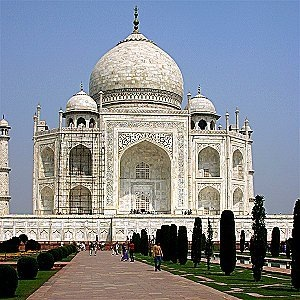
\includegraphics{images/gimp_original}
    \end{subfigure}%
    %
    \begin{subfigure}{0.5\textwidth}
    \centering
    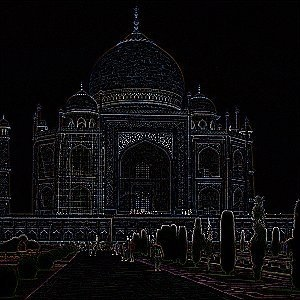
\includegraphics{images/gimp_edgedetect}
    \end{subfigure}

\caption{A demonstration of an edge-detecting convolution, from the GIMP User's Manual. \cite{gimpconvolution}}
\label{fig:gimp_edge}
\end{figure}

Convolutional neural networks are therefore the product of using these 

% overparametrization




\chapter{Related Works}

In this work, we are primarily interested in optimizing neural network architectures and other hyperparameters.
Towards this end, we investigate current findings in the literature.
Neural network architecture self-optimization is a very new topic, and many results are preliminary or incomplete.
Nevertheless, they provide an important glimpse into the contemporary research space, and are highly motivational to the specific topic of this thesis.
The aim of this section is to cover some of the existing work that specifically focuses on network optimization, and to provide some grounding for our contributions.

\section{Parameter Deletion}
Ever since neural networks have been developed, experts have wondered how to make them more efficient.
The fixed initial structure required to train a network is one that is inherently overparametrized, because the minimum number of parameters needed is not known ahead of time.
Further exacerbating the problem, neural network training is often slow and requires significant computational power, limiting the ability to test out how altering the number of parameters affects the network results.
The natural solution is, therefore, to train an oversized network, and then whittle it down to size.
Initial practices were based on heuristic deletion; that is, algorithms that deleted all weights $w$ where $w < p$ for some low-pass filter $p$.
These methods generally result in a sparse network (where the network has missing connections), which are difficult to represent and operate on efficiently.

LeCun et al.'s early work from 1989, \emph{Optimal Brain Damage} \cite{lecun1989optimal}, showed that these heuristic-based methods were inefficient and could irreparably destroy a network.
They proposed a method based on error gradients that could more accurately find weights that can be removed with minimal perturbation to the final error.
By what is effectively the butterfly effect, the deletion of a weight with small magnitude can actually prove to have a significant impact on the network.
By taking the Taylor series of the error function to two terms, they show that it is possible to calculate the two-dimensional Hessian matrix representing the importance of each weight.
For reasons of efficiency, LeCun et al. approximate the Hessian with a diagonal matrix, and gradually remove the terms with the smallest saliency.
By retraining the network repeatedly after removing connections, they are able to show a significant improvement in performance despite requiring less parameters.

This was taken a step further by Hassibi et al. \cite{hassibi1993second} in their followup work, \emph{Optimal Brain Surgeon}.
By analyzing the Hessian matrix of typical networks, they show that the Hessian matrix is often nondiagonal, and that Optimal Brain Damage can often irreparably destroy small networks.
They utilize the full Hessian matrix to better understand the interactions between each pair of weights.
Hassibi et al.'s algorithm is among the most detailed methods shown to delete weights from a network, and they find that their algorithm is in fact optimal for specific small networks.
However, the calculation of the Hessian is an $O(n^2)$ operation in both space and time, making it largely unsuitable for networks in the modern age, where $n$ (the number of parameters) is often in the millions or tens of millions.

Within the last few years, an increasing amount of literature has been published on parameter deletion, especially as network complexity has grown at a pace that far outpaces the corresponding technological advancements.
Han et al. \cite{han2015learning} work on reducing existing architectures using a combination of heuristic-based deletion methods and weight regularization, and show that there is significant promise.
These methods are more common and rely on deleting weights, which can help optimize performance when running on CPUs.
They have limited application on GPUs and especially on convolutions.
To solve this problem, Hu et al. \cite{hu2016network} trim entire nodes and convolutions from the network, allowing better performance by fully removing them from the layers.
They improve on Han et al.'s results by producing networks that are smaller and more accurate, and are even able to see some extremely small improvements over the untrimmed network for some of the largest networks.
They hypothesize that this is due to optimizer efficiency.
However, we note that despite showing that it is possible to reduce parameter count significantly, no modern work has measurably better overall results.
These results are further supported by Murray and Chiang \cite{murray2015auto}, who utilize the same methodologies on natural language modelling and observe similar performance.
Instead, the goal is generally to minimize model size while keeping accuracy fixed (or reducing it slightly).
In this thesis, we aim to more efficiently utilize existing capacity and achieve improved results over the architectures we start with.

\section{Specialized Architectures}
Another direction researchers have exploited to minimize the number of parameters required is specialized network design.
Notable work in this field includes Squeezenet \cite{iandola2016squeezenet} by Iandola et al., which utilizes a number of space-saving tricks to produce a network which has 50 times less parameters.
Courbariaux and Bengio further demonstrate that it is possible to constrain a network entirely to binary weights and activations (either $+1$ or $-1$) without significant loss in accuracy.
Using this method, they are able to construct a convolutional neural network, and optimize it for CPU performance to achieve competitive results.
These results are largely corroborated by Rastegari et al. \cite{rastegari2016xnor}, who also use a binarized network and significant usage of the XNOR operation to optimize a wider variety of modern networks.
It is important to note, however, that the performance of these methods is still insufficient to reliably overtake GPU networks.
Courbariaux and Bengio perform their training against ``an unoptimized GPU kernel'', while Rastegari et al. perform an efficiency investigation but do not discuss raw performance.
While such approaches hint at future promise, in their current state they are more complicated and are still far from seeing general use in modern libraries.

On the other hand, it is not necessary to impose such harsh limits on the network in order to find areas of improvement.
Google's Inception network \cite{szegedy2015going}, developed by Szegedy et al., has gone through various iterations, which all involve complex pooling of different convolutional kernel sizes.
In their 2016 update to the architecture \cite{szegedy2016rethinking}, they focus on tuning the inefficiently large filter sizes used in the previous revision.
They note that a $5\times 5$ convolution is effectively the same (covers the same area) as two $3\times 3$ convolutions while requiring more parameters (25 versus $9 \cdot 2 = 18$), dubbing this reduction as filter factorization.
In the same vein, it is possible to reduce a $3\times 3$ convolution to a $3\times 1$ convolution followed by a $1\times 3$ convolution, which requires a third less parameters.

There are various benefits to an increased number of smaller layers over one larger layer beyond parameter reduction.
Reducing the number of layers allows for the increased application of nonlinear activation functions, which are generally regarded as critical for learning complex problems.
Furthermore, it allows an increased number of layers with the same number of parameters.
Most networks are primarily limited by memory, especially as modern training algorithms require a 
Even though inference is generally more efficient, it can still remain a difficult problem for more constrained hardware; part of Squeezenet's contribution was the possibility of reducing a model to a size that could be run on modern FPGAs.

\section{Network Expansion}
The counterpart to parameter deletion is network expansion, which tries to add parameters and learning capacity to a network dynamically.
One of the important works in this field is Cascade-Correlation Learning by Fahlman and Lebiere \cite{fahlman1990cascade}, which fixes a network and gradually adds single nodes to the network at a time.
Their proposed network learns without backpropagation but rather through adding new nodes in order to correct for error.
We derive some inspiration for our algorithm in Fahlman and Lebiere's interesting link between introduction of learning capacity and freezing the original network.
The main difficulty with their specific algorithm is that it depends on adding individual nodes, which would be prohibitively slow to generate the network sizes that are common in the modern age.
Additionally, we are unaware of any existing work that utilizes their findings in a way that is able to take advantage of convolutions.

An alternative way of thinking about this problem was tackled by Chen et al. They develop Net2Net \cite{chen2015net2net}, which takes a pretrained smaller network and allows a partial transfer of these learned weights to an expanded network.
Noting that modern deep learning research usually requires the training of a number of different networks, they develop an architecture to minimize the amount of repeated computation, and are able to achieve improved results on the ImageNet dataset.

In general, network expansion is an understudied topic in the modern literature, and we believe that there is significant room for improvement, especially with regards to modern deep networks.
We aim to provide a form of this by introducing dynamic network capacity, which allows layers to resize up to a fixed size during runtime.


\chapter{Methodology}
In this section, we provide a description of the algorithms we propose.
We construct a network structure that allows dynamic resizing and freezing, which has not been investigated on this scale before in the literature.
We further develop this algorithm to per-layer capacity tuning, which we note can help ensure that every layer is being utilized optimally.
We then discuss the process of our implementation and a variety of surrounding details.

\section{Dynamic Network Capacity}
Network design has almost always focused on preferring overparametrization; this principle is clear because underparametrized networks, by definition, simply cannot learn the problem.
Our method involves defining the network in such a way that network capacity can be expandewith minimal overparametrization. way that, to the best of our knowledge, is unique in the literature.
This allow a network to be undersized initially, but gradually gain the necessary capacity with minimal overparametrization.
In particular, it allows per-layer expansion during runtime while keeping the weights that have already been trained, and performs this efficiently.
While this requires upfront allocation of the maximum potential capacity due to library constraints, these requirements are not set in stone.
Furthermore, it is generally desirable to train smaller networks if possible, due to increased speed and less chance of overfitting errors.
As such, we rework well-known architectures to allow dynamic capacity, which requires a higher-level framework that keeps track of all layer sizes to ensure consistent inputs and outputs.
In particular, because we explore shortcuts connections as seen in residual networks, this involves holding the necessary structure to ensure that the shortcut is projected to the correct dimension.

For determining how the network should begin to utilize the ability to modify capacity dynamically, in this thesis we focus primarily on expansion.
We track the moving average of error rates and gradually resize the network as the error plateaus (indicating that it has been trained to capacity).
This process requires a few new hyperparameters to tune the definition of an error plateau, but allows some other ones, such as  precise network sizing, to be masked away.
We argue that this is a highly beneficial development for deep learning, as it represents a far more visible approach to network architecture as error rates are clear and interpretable.
In contrast, beyond some vague sense that larger networks can learn harder problems, the motivation for choosing specific network sizes remains generally unclear.
Within the field of residual networks alone, results have been published both demonstrating the superiority of prioritizing depth and prioritizing width, leading to a very murky situation.


\section{Fixed Networks}
Parameter count is a difficult problem to solve, and one that is especially complicated because it is difficult to remove weights from a network while maintaining efficiently dense connections.
Rather than deal with the numerous details required here, we regard a different way of modifying the trainable network capacity by freezing parts of the network after they have converged.
While this does not decrease model size, it improves the number of parameters that need to be trained, which is a potential point of efficiency.
We note that this can be more useful than parameter deletion, as sparse networks are not very well supported by deep learning libraries, thus oftentimes necessitating that the ``deleted'' parameters remain in the model but fixed to zero.
This allows the network to utilize the capacity it has learned but avoids calculating a substantial number of gradients, optimizing the bottleneck of the training process.
This additionally prevents the network from shifting excessively over time, a problem much like the covariate shift that is often covered by batch normalization.

\section{Layer-Specific Analysis}
In the original paper on Residual Networks, He et al. analyze the relative strengths of each layer activation.
To perform this analysis, they record the activations over a minibatch and perform aggregate statistics.
In particular, they focus on the standard deviation of the layers as a measure of the relative amount of information in each layer, where the mean is less informative as it is largely influenced by the bias terms of the network.
We aim to utilize this methodology to determine where extra capacity is useful.
Noting that the standard deviation is not constant across layers, we note that these layers are likely producing more contribution to the end result.
While this is beneficial, it may also mean that there is an opportunity to increase the capacity of these layers.
He et al.'s analysis indicates that deeper networks have lower activation strength in general, which we can observe to also be smoother.
We seek to encourage this property by expanding the residual blocks that have the highest activations, noting especially that they tend to occur when the network downsamples the image.

\section{Implementation}
We performed all of our experiments within Google's Tensorflow \cite{abadi2016tensorflow} framework.
Tensorflow imposes a style of computation which is not immediately adaptable to our experiments, but it was nevertheless chosen due to its prevalence within the current literature. 
Its popularity has largely affected the number of open-source code samples available, and many current architectures have clear examples in Tensorflow.
The thriving ecosystem of open-source contributions around Tensorflow proved to be a highly beneficial factor in providing a variety of existing architectures for experimentation.

As was noted before, Tensorflow operates in a slightly different way than many other libraries.
Rather than allowing the user to chain together operations at random, it fixes a computational graph which defines the full model.
Google's developers preferred this static model as it is generally well-suited to a lot of deep learning research, while also being flexible enough to allow for distributed computing (of crucial importance to a a cloud company like Google).
This, however, poses an obvious problem with our algorithm, which is largely dynamic.
Therefore, we had to develop a number of workarounds in order to interface with the static computational graph.
While it is possible to use conditional blocks to disable parts of the graph, it is impossible to insert layers or other capacity during runtime.
As such, the entire possible network capacity has to be allocated upfront, which potentially reduces the range of experimentation.
This additionally means that while parts of the network can be disabled, they still take important parameter space which cannot be reallocated to other parts of the network.

Other libraries were explored briefly, but they either did not provide the necessary flexibility or lacked a reasonable set of tutorials/examples to facilitate the work within this thesis.
For example, one of the more common tools in image-based deep learning has been Caffe \cite{jia2014caffe}, which boasts well-tuned performance as well as a public repository of models in the Caffe Model Zoo.
Unfortunately, since Caffe is written almost entirely in C++, it is largely unamenable to testing and infrastructure development.
Modifying Caffe to implement new training methods typically requires a significant contribution in C++, which requires an overhead not often undertaken except by researchers with significant prior experience.
Furthermore, models are loaded in a fixed format, which hampers the ability to dynamically redefine networks.
On the other side of the spectrum are libraries like Keras, which usually serve as a higher-level wrapper to other deep learning libraries.
They were generally judged as being insufficiently expressive for the type of modifications we performed, so we considered other options.

All experimentation was performed on a GTX 1060, which was provided via a grant from Princeton SEAS.
In recent years, GPU computation has become the standard for deep learning computation, as it can increase performance by nearly an order of magnitude.
Particularly for models like modern residual networks, which can take days to converge to reasonable accuracy, it is nearly impossible to train neural networks on CPU servers.
Tensorflow still utilizes the CPU extensively to coordinate training and perform a significant amount of calculations, but modern-day GPUs are nearly perfectly designed for the type of computations required for convolutions.

A recent glut of libraries aimed at helping automate the deep learning deployment process has led to a variety of different software packages.
NVIDIA's CUDA and CUDNN libraries, both of which are crucial for the performance of modern deep learning libraries, require a complex set of dependencies and installation procedures.
To automate these processes, NVIDIA has recently released the \texttt{nvidia-docker} tool, which provides an abstraction on top of Docker that is designed to expose the GPU without requiring a complex installation method for the requisite GPU drivers.
We use this library to deploy CUDNN v5, as well as the latest GPU drivers and Tensorflow version as of this writing (375.39 and 1.1.0-rc0, respectively).

As Tensorflow's interface is best utilized in Python, we performed some initial testing with the Jupyter application.
Jupyter exposes a dynamic notebook interface that allows ``cells'' of code to be run in an interactive instance, which also shows outputs inline.
Despite being relatively useful for basic prototyping, the largely static nature of Tensorflow's graph structure meant that for the larger tests, there was little to no developer-side improvement over traditional coding, which we eventually reverted to.
Nevertheless, we note that Jupyter is a useful interface for demonstrating concepts, as many Tensorflow code examples online are in Jupyter \texttt{.ipynb} format.
In particular, GitHub supports native inline presentation of Jupyter notebooks, which proved to be far more efficient than the typical workflow of downloading code examples, waiting for execution, and parsing terminal output which is often difficult to link to specific code sections.
This allows us to cleanly adapt existing code, which helped significantly when doing intial development of the experiments.

\subsection{Implementation Details \& Notes}
Throughout our experiments, we utilize the Adam optimizer developed by Kingma and Ba \cite{kingma2014adam} as it allows adaptive training without requiring the careful learning rate tuning that is generally required for straightforward gradient-descent optimization.
Many typical optimizers require handholding through epochs to achieve optimal results, while the default parameters for Adam allow far less supervision.
In particular, hyperparameter search can often involve determining the correct timings of when to drop learning rate, which ``slows'' the network's training but also serves to stabilize it.
As we aim for our algorithm to be as high-level as possible, this represents yet another dimension of optimization, which lies outside of the scope this thesis.

We also rely on Glorot and Bengio's Xavier initializer \cite{glorot2010understanding} to initialize the weights of the network, as it is a common improvement over typical random initialization, but is still relatively simple to use.
This poses a small relevant side note to our algorithm; because only parts of the network are initially exposed, the initializer is potentially using incorrect values.
Network initialization is crucial to achieving good results (one of the famous papers is this field is humorously entitled \emph{All you need is a good init} \cite{mishkin2015all}), and these initializers are dependent on the shape of the variable to determine properties like the variance of a random distribution.
Due to the lack of dynamic initialization in Tensorflow, we do not investigate this issue further.
Future work may include developing a custom initializer for this problem.

We fix portions of the network by using Tensorflow's \texttt{tf.stop\_gradient} method.
Support for freezing whole layers is a generally universal feature across deep learning libraries, but our investigation showed that none supported partial freezing---that is, the ability to train part of a layer while keeping the other part fixed.
Notably, because we need to modify the amount of the layer that is fixed during runtime, it is impossible to decompose this problem into two separate layers.
Our implementation involves deconstructing a variable into slices before reassembling it; a quick demonstration in pseudocode is presented in Listing~\ref{lst:var_deconst}.
This kind of workaround for a lack of inbuilt dynamicism is a typical example of what was necessary to build the desired structure into Tensorflow.

\begin{lstlisting}[caption={Variable Deconstruction}, label={lst:var_deconst}, captionpos=b]
# x:              input, full-size variable
# fix_capacity:   what portion of x to freeze
# train_capacity: what porition of x to train,
#                 assumed to be greater than fix_capacity
f(x, fix_capacity, train_capacity):
    # slice X according to each capacity
    fixed = x[:fix_capacity]
    train = x[fix_capacity:train_capacity]

    # freeze fixed
    fixed = stop_gradient(fixed)

    # reassemble 
    new_x = concat(fixed, train)

    return new_x
\end{lstlisting}

In following with a common Tensorflow workflow, we separate the testing and training models rather than running them under the same code but with different inputs.
This has the key benefit of allowing inference testing to be completely independent of the training loop.
In our case, this allows us to run inference on the CPU, as it is both less computationally intensive and less time dependent; we note that this could be further extended to allow the testing dataset to be run on a completely different machine.
However, this practice also comes with a few downsides, as training error becomes largely separated from testing error.
Without careful matching of the epoch count between the two methods, it becomes impossible to compare the two except during runtime observation.
We did not perform this matching due to a lack of time, so we do not report training and testing errors on the same timescales for our results.
We believe our current data is sufficiently representative of our algorithm, but note that this could allow more discussion on generalizability metrics, which we expand on in a later section.

\chapter{Experiments}
In this section, we present our findings.
We expect that our algorithm will improve the training process for a regular deep learning user, both in the perspective of training performance and in final accuracy.
This hypothesis is borne out in the smaller datasets, but remains somewhat inconclusive for larger datasets.
Nevertheless, we note that there are significant points of interest that are raised as a result, and the potential for improvement on this algorithm is encouraging.

\section{Function Regression}
Our first experiment is relatively simplistic, but is also indicative of the basic algorithm's performance.
In this experiment, we approximate the trigonometric sine function in the range of $[-2\pi, 2\pi]$.
Our architecture for this experiment is extremely simple: it is merely a feedforward network with one hidden layer consisting of up to 500 nodes.
This is sufficient capacity to learn the sine function with great accuracy, but can still be heavily affected by the training regime applied to it.
We investigate the importance of the hidden layer's capacity by testing static networks of 100 and 500 nodes, then compare these results to a dynamically sizing network.

For this experiment, we split the network into fifths, and initialize them all before any training begins.
We initially only let the network use the first fifth of its capacity, making it equivalent to the 100-node static test.
We track the moving average of the error, and after it fails to rise within the last 10 batches, we proceed to increase the capacity of the network by a fifth, but also freeze the existing capacity.
This serves to force the additional capacity to learn the mistakes of the existing capacity, rather than just adding additional parameters that would change alongside the original.
We see the results of the experiment in Figure~\ref{fig:sin_loss}, in which our method is labelled ``adaptive.''

\begin{figure}[!htb]
\centering
\resizebox{0.8\textwidth}{!}{% GNUPLOT: LaTeX picture with Postscript
\begingroup
  \makeatletter
  \providecommand\color[2][]{%
    \GenericError{(gnuplot) \space\space\space\@spaces}{%
      Package color not loaded in conjunction with
      terminal option `colourtext'%
    }{See the gnuplot documentation for explanation.%
    }{Either use 'blacktext' in gnuplot or load the package
      color.sty in LaTeX.}%
    \renewcommand\color[2][]{}%
  }%
  \providecommand\includegraphics[2][]{%
    \GenericError{(gnuplot) \space\space\space\@spaces}{%
      Package graphicx or graphics not loaded%
    }{See the gnuplot documentation for explanation.%
    }{The gnuplot epslatex terminal needs graphicx.sty or graphics.sty.}%
    \renewcommand\includegraphics[2][]{}%
  }%
  \providecommand\rotatebox[2]{#2}%
  \@ifundefined{ifGPcolor}{%
    \newif\ifGPcolor
    \GPcolorfalse
  }{}%
  \@ifundefined{ifGPblacktext}{%
    \newif\ifGPblacktext
    \GPblacktexttrue
  }{}%
  % define a \g@addto@macro without @ in the name:
  \let\gplgaddtomacro\g@addto@macro
  % define empty templates for all commands taking text:
  \gdef\gplbacktext{}%
  \gdef\gplfronttext{}%
  \makeatother
  \ifGPblacktext
    % no textcolor at all
    \def\colorrgb#1{}%
    \def\colorgray#1{}%
  \else
    % gray or color?
    \ifGPcolor
      \def\colorrgb#1{\color[rgb]{#1}}%
      \def\colorgray#1{\color[gray]{#1}}%
      \expandafter\def\csname LTw\endcsname{\color{white}}%
      \expandafter\def\csname LTb\endcsname{\color{black}}%
      \expandafter\def\csname LTa\endcsname{\color{black}}%
      \expandafter\def\csname LT0\endcsname{\color[rgb]{1,0,0}}%
      \expandafter\def\csname LT1\endcsname{\color[rgb]{0,1,0}}%
      \expandafter\def\csname LT2\endcsname{\color[rgb]{0,0,1}}%
      \expandafter\def\csname LT3\endcsname{\color[rgb]{1,0,1}}%
      \expandafter\def\csname LT4\endcsname{\color[rgb]{0,1,1}}%
      \expandafter\def\csname LT5\endcsname{\color[rgb]{1,1,0}}%
      \expandafter\def\csname LT6\endcsname{\color[rgb]{0,0,0}}%
      \expandafter\def\csname LT7\endcsname{\color[rgb]{1,0.3,0}}%
      \expandafter\def\csname LT8\endcsname{\color[rgb]{0.5,0.5,0.5}}%
    \else
      % gray
      \def\colorrgb#1{\color{black}}%
      \def\colorgray#1{\color[gray]{#1}}%
      \expandafter\def\csname LTw\endcsname{\color{white}}%
      \expandafter\def\csname LTb\endcsname{\color{black}}%
      \expandafter\def\csname LTa\endcsname{\color{black}}%
      \expandafter\def\csname LT0\endcsname{\color{black}}%
      \expandafter\def\csname LT1\endcsname{\color{black}}%
      \expandafter\def\csname LT2\endcsname{\color{black}}%
      \expandafter\def\csname LT3\endcsname{\color{black}}%
      \expandafter\def\csname LT4\endcsname{\color{black}}%
      \expandafter\def\csname LT5\endcsname{\color{black}}%
      \expandafter\def\csname LT6\endcsname{\color{black}}%
      \expandafter\def\csname LT7\endcsname{\color{black}}%
      \expandafter\def\csname LT8\endcsname{\color{black}}%
    \fi
  \fi
    \setlength{\unitlength}{0.0500bp}%
    \ifx\gptboxheight\undefined%
      \newlength{\gptboxheight}%
      \newlength{\gptboxwidth}%
      \newsavebox{\gptboxtext}%
    \fi%
    \setlength{\fboxrule}{0.5pt}%
    \setlength{\fboxsep}{1pt}%
\begin{picture}(7200.00,5040.00)%
    \gplgaddtomacro\gplbacktext{%
      \csname LTb\endcsname%
      \put(1210,1374){\makebox(0,0)[r]{\strut{}$0.0001$}}%
      \put(1210,1829){\makebox(0,0)[r]{\strut{}$0.001$}}%
      \put(1210,2284){\makebox(0,0)[r]{\strut{}$0.01$}}%
      \put(1210,2740){\makebox(0,0)[r]{\strut{}$0.1$}}%
      \put(1210,3195){\makebox(0,0)[r]{\strut{}$1$}}%
      \put(1210,3650){\makebox(0,0)[r]{\strut{}$10$}}%
      \put(1210,4105){\makebox(0,0)[r]{\strut{}$100$}}%
      \put(1342,1154){\makebox(0,0){\strut{}$0$}}%
      \put(1888,1154){\makebox(0,0){\strut{}$10$}}%
      \put(2434,1154){\makebox(0,0){\strut{}$20$}}%
      \put(2980,1154){\makebox(0,0){\strut{}$30$}}%
      \put(3526,1154){\makebox(0,0){\strut{}$40$}}%
      \put(4073,1154){\makebox(0,0){\strut{}$50$}}%
      \put(4619,1154){\makebox(0,0){\strut{}$60$}}%
      \put(5165,1154){\makebox(0,0){\strut{}$70$}}%
      \put(5711,1154){\makebox(0,0){\strut{}$80$}}%
      \put(6257,1154){\makebox(0,0){\strut{}$90$}}%
      \put(6803,1154){\makebox(0,0){\strut{}$100$}}%
    }%
    \gplgaddtomacro\gplfronttext{%
      \csname LTb\endcsname%
      \put(176,2739){\rotatebox{-270}{\makebox(0,0){\strut{}log loss}}}%
      \put(4072,824){\makebox(0,0){\strut{}epoch}}%
      \csname LTb\endcsname%
      \put(5816,3932){\makebox(0,0)[r]{\strut{}100-node static}}%
      \csname LTb\endcsname%
      \put(5816,3712){\makebox(0,0)[r]{\strut{}500-node static}}%
      \csname LTb\endcsname%
      \put(5816,3492){\makebox(0,0)[r]{\strut{}adaptive}}%
    }%
    \gplbacktext
    \put(0,0){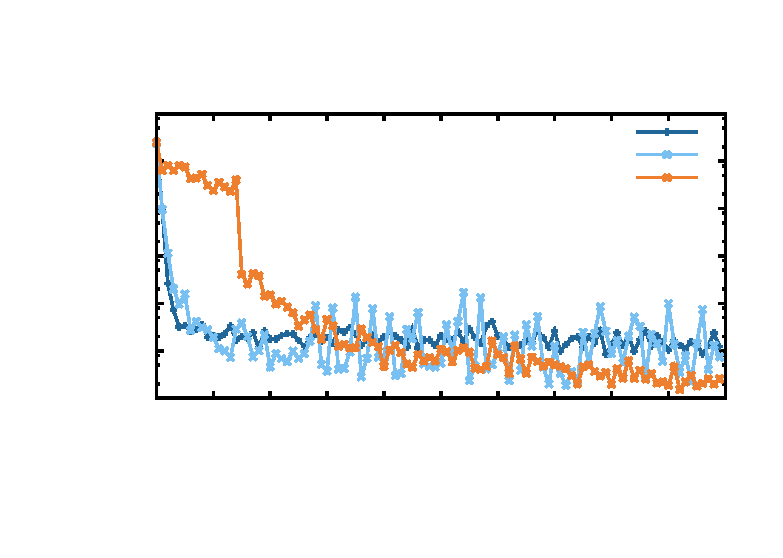
\includegraphics{sin}}%
    \gplfronttext
  \end{picture}%
\endgroup
}
\caption{Sine function approximation by different methods.}
\label{fig:sin_loss}
\end{figure}

It is immediately clear that our method is able to converge to a much better solution than simple training methods.
Importantly, we plot the y-axis on the logarithmic scale, so small improvements are in fact extremely significant.
Firstly, we note that increasing the capacity of the network from 100 to 500 nodes does not have a significant impact on final error.
In fact, the 500-node result would generally be considered worse, as it exhibits far noisier behavior.
On quick inspection, the adaptive method is generally superior in every way.
Surprisingly, however, the adaptive network is initially slower to train compared to the 100-node network, despite utilizing same capacity. 
We suspect this difference has to do with the potential variances in optimizer and initializer performance discussed above.
Regardless of its early-stage performance, we can see that it benefits tremendously from increased capacity, and overtakes the both of the static networks by around epoch 35.
There are some small spikes in error which we attribute to the sudden increase in capacity, but overall the performance is consistently better than that of the static methods.

\begin{table}[!htb]
\centering
\caption{Final-10 errors for various methods.}
\label{table:sin_errors}
\begin{tabular}{@{}lrr@{}}
\toprule
Network  & Mean    & Standard Deviation \\ \midrule
100-node & 0.00138 & 0.000389           \\
500-node & 0.00234 & 0.003261           \\
Adaptive & 0.00024 & 0.000084           \\ \bottomrule
\end{tabular}
\end{table}

To measure these results quantitatively, we consider both the average and the standard deviations of loss over the final 10 samples.
These results are presented in Table~\ref{table:sin_errors}.
We can see that the noisier results of the 500-node network are actually noticeably worse when averaged---it has nearly twice the error of the smaller 100-node network.
Furthermore, the standard deviation is an order of magnitude larger over the 100-node network., which is extremely poor as it is larger than the average error.
In contrast, the adaptive method exhibits both lower mean and standard deviation in the long run.
This indicates an improvement not just in learning capacity, but also in stability, which is a crucial property for training as noisy behavior is indicative of a number of other problems.
Chief amongst these is the simple problem that noisy behavior makes it difficult to decide when an experiment has concluded.
In any case, throughout this experiment, the adaptive method has offered significant improvements in performance over either static network.

\section{MNIST Classifier}
Modern deep learning algorithms have generally tended to be developed for image classification purposes, in part due to the original usage of convolutional neural networks.
LeCun et al.'s original work with CNNs \cite{lecun1998gradient} was in designing a classifier for the MNIST dataset, a collection of monochrome handwritten digits.
These images have been preprocessed for regularity, and have all been resized to a standard $28\times 28$ resolution.
MNIST is a well-regarded small image classification dataset which serves as a useful benchmark for this algorithm.


Tensorflow includes MNIST support as part of the base installation as part of its example code, so we are able to rely on a simple interface to download, load, and process the image data according to standard image augmentation purposes.
For the purposes of this experiment, we follow the example convolutional neural network provided by Google \cite{deepmnist}, and modify it so we can apply our expansion algorithm.
This is a typical structure, with two convolutional layers utilizing $7\times 7$ kernels, and then a fully-connected layer of 1024 nodes.
While this is far from the best known architectures for MNIST, it serves as a good baseline and is easily accessible.
Once again, we apply our methodology of training the network in portions.
This time, due to the increased capacity of the network, we instead train it in tenths, once again expanding when the moving average of accuracy begins to stall or decrease.

\begin{figure}[!htb]
\centering
\resizebox{0.8\textwidth}{!}{% GNUPLOT: LaTeX picture with Postscript
\begingroup
  \makeatletter
  \providecommand\color[2][]{%
    \GenericError{(gnuplot) \space\space\space\@spaces}{%
      Package color not loaded in conjunction with
      terminal option `colourtext'%
    }{See the gnuplot documentation for explanation.%
    }{Either use 'blacktext' in gnuplot or load the package
      color.sty in LaTeX.}%
    \renewcommand\color[2][]{}%
  }%
  \providecommand\includegraphics[2][]{%
    \GenericError{(gnuplot) \space\space\space\@spaces}{%
      Package graphicx or graphics not loaded%
    }{See the gnuplot documentation for explanation.%
    }{The gnuplot epslatex terminal needs graphicx.sty or graphics.sty.}%
    \renewcommand\includegraphics[2][]{}%
  }%
  \providecommand\rotatebox[2]{#2}%
  \@ifundefined{ifGPcolor}{%
    \newif\ifGPcolor
    \GPcolorfalse
  }{}%
  \@ifundefined{ifGPblacktext}{%
    \newif\ifGPblacktext
    \GPblacktexttrue
  }{}%
  % define a \g@addto@macro without @ in the name:
  \let\gplgaddtomacro\g@addto@macro
  % define empty templates for all commands taking text:
  \gdef\gplbacktext{}%
  \gdef\gplfronttext{}%
  \makeatother
  \ifGPblacktext
    % no textcolor at all
    \def\colorrgb#1{}%
    \def\colorgray#1{}%
  \else
    % gray or color?
    \ifGPcolor
      \def\colorrgb#1{\color[rgb]{#1}}%
      \def\colorgray#1{\color[gray]{#1}}%
      \expandafter\def\csname LTw\endcsname{\color{white}}%
      \expandafter\def\csname LTb\endcsname{\color{black}}%
      \expandafter\def\csname LTa\endcsname{\color{black}}%
      \expandafter\def\csname LT0\endcsname{\color[rgb]{1,0,0}}%
      \expandafter\def\csname LT1\endcsname{\color[rgb]{0,1,0}}%
      \expandafter\def\csname LT2\endcsname{\color[rgb]{0,0,1}}%
      \expandafter\def\csname LT3\endcsname{\color[rgb]{1,0,1}}%
      \expandafter\def\csname LT4\endcsname{\color[rgb]{0,1,1}}%
      \expandafter\def\csname LT5\endcsname{\color[rgb]{1,1,0}}%
      \expandafter\def\csname LT6\endcsname{\color[rgb]{0,0,0}}%
      \expandafter\def\csname LT7\endcsname{\color[rgb]{1,0.3,0}}%
      \expandafter\def\csname LT8\endcsname{\color[rgb]{0.5,0.5,0.5}}%
    \else
      % gray
      \def\colorrgb#1{\color{black}}%
      \def\colorgray#1{\color[gray]{#1}}%
      \expandafter\def\csname LTw\endcsname{\color{white}}%
      \expandafter\def\csname LTb\endcsname{\color{black}}%
      \expandafter\def\csname LTa\endcsname{\color{black}}%
      \expandafter\def\csname LT0\endcsname{\color{black}}%
      \expandafter\def\csname LT1\endcsname{\color{black}}%
      \expandafter\def\csname LT2\endcsname{\color{black}}%
      \expandafter\def\csname LT3\endcsname{\color{black}}%
      \expandafter\def\csname LT4\endcsname{\color{black}}%
      \expandafter\def\csname LT5\endcsname{\color{black}}%
      \expandafter\def\csname LT6\endcsname{\color{black}}%
      \expandafter\def\csname LT7\endcsname{\color{black}}%
      \expandafter\def\csname LT8\endcsname{\color{black}}%
    \fi
  \fi
    \setlength{\unitlength}{0.0500bp}%
    \ifx\gptboxheight\undefined%
      \newlength{\gptboxheight}%
      \newlength{\gptboxwidth}%
      \newsavebox{\gptboxtext}%
    \fi%
    \setlength{\fboxrule}{0.5pt}%
    \setlength{\fboxsep}{1pt}%
\begin{picture}(7200.00,5040.00)%
    \gplgaddtomacro\gplbacktext{%
      \csname LTb\endcsname%
      \put(1078,1341){\makebox(0,0)[r]{\strut{}$0.001$}}%
      \put(1078,2273){\makebox(0,0)[r]{\strut{}$0.01$}}%
      \put(1078,3206){\makebox(0,0)[r]{\strut{}$0.1$}}%
      \put(1078,4138){\makebox(0,0)[r]{\strut{}$1$}}%
      \put(1210,1121){\makebox(0,0){\strut{}$0$}}%
      \put(1769,1121){\makebox(0,0){\strut{}$100$}}%
      \put(2329,1121){\makebox(0,0){\strut{}$200$}}%
      \put(2888,1121){\makebox(0,0){\strut{}$300$}}%
      \put(3447,1121){\makebox(0,0){\strut{}$400$}}%
      \put(4007,1121){\makebox(0,0){\strut{}$500$}}%
      \put(4566,1121){\makebox(0,0){\strut{}$600$}}%
      \put(5125,1121){\makebox(0,0){\strut{}$700$}}%
      \put(5684,1121){\makebox(0,0){\strut{}$800$}}%
      \put(6244,1121){\makebox(0,0){\strut{}$900$}}%
      \put(6803,1121){\makebox(0,0){\strut{}$1000$}}%
    }%
    \gplgaddtomacro\gplfronttext{%
      \csname LTb\endcsname%
      \put(176,2739){\rotatebox{-270}{\makebox(0,0){\strut{}log loss}}}%
      \put(4006,791){\makebox(0,0){\strut{}epoch}}%
      \csname LTb\endcsname%
      \put(5816,3965){\makebox(0,0)[r]{\strut{}adaptive}}%
      \csname LTb\endcsname%
      \put(5816,3745){\makebox(0,0)[r]{\strut{}standard}}%
    }%
    \gplbacktext
    \put(0,0){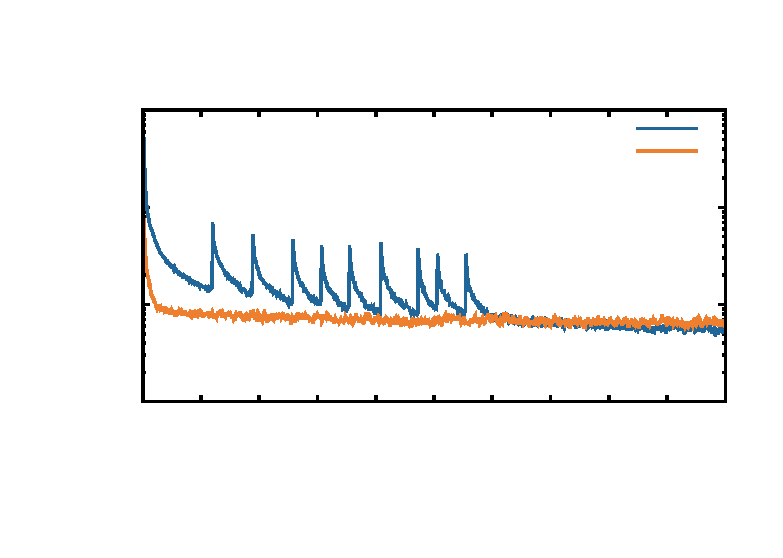
\includegraphics{mnist}}%
    \gplfronttext
  \end{picture}%
\endgroup
}
\caption{MNIST loss trained by different methods.}
\label{fig:mnist_loss}
\end{figure}

We show the results of the MNIST classifier in Figure~\ref{fig:mnist_loss}.
In this experiment, there are significant spikes to the loss when new capacity is added, indicating that the extra capacity produces a significant shock on the network.
We hypothesize that this is due to the fact that multiple layers are all increasing in capacity simultaneously, which leads to a much more pronounced change in outputs.
Whereas the previous experiment only involved a single layer, the interactions of additional units that are connected to the original network changes the dynamics significantly.
This still shows an improvement over the standard network, although the difference is much smaller than previously demonstrated.
This is likely due to the fact that the error is very low in both examples; typical algorithms achieve over 99\% accuracy on MNIST.
It appears that the adaptive network is still improving over time but may be limited by the length of the experiment, while the standard network has converged to its best potential.
We were not able to test this theory more fully due to time constraints, but leave it as a potential point of interest.
We also report the mean and standard deviation statistics for this experiment in Table~\ref{table:mnist_errors}. 
This corroborates the close performance between the two networks, but also demonstrates the improvements our adaptive method produces over a standard network of the same final size.
Both the error and the standard deviation are lower, indicating a mild improvement.

\begin{table}[!htb]
\centering
\caption{Comparison on MNIST.}
\label{table:mnist_errors}
\begin{tabular}{@{}lrr@{}}
\toprule
Network  & Mean    & Standard Deviation \\ \midrule
standard & 0.00686 & 0.000369           \\
adaptive & 0.00633 & 0.000248           \\ \bottomrule
\end{tabular}
\end{table}


\section{CIFAR-100}
One of the common modern image classification datasets is CIFAR-100, a set of 60000 images collected by researchers at the University of Toronto.
It consists of 20 classes, each with 5 subclasses.
For each of the 100 subclasses, there are 500 training images and 100 testing images.
The images are in color, but are of low resolution at $32\times 32$; the small size of the dataset makes it especially attractive as an experimental problem; a few sample images are shown in Figure~\ref{fig:cifar100}.
Larger image classification datasets exist, such as the commonly used ImageNet, but due to its over 150GB download size and consequently longer training times, it was not considered for this thesis.
Most modern deep learning papers include results on both CIFAR-10 (a smaller version of the same problem) and CIFAR-100; we choose CIFAR-100 as state of the art performance on CIFAR-10 is over 90\%, leading to a closer and less separable grouping of experimental results.
In doing this, we hope to avoid the problem seen on the MNIST dataset, where it is extremely difficult to improve on results that are already nearly perfect.

\begin{figure}[!htb]
\centering
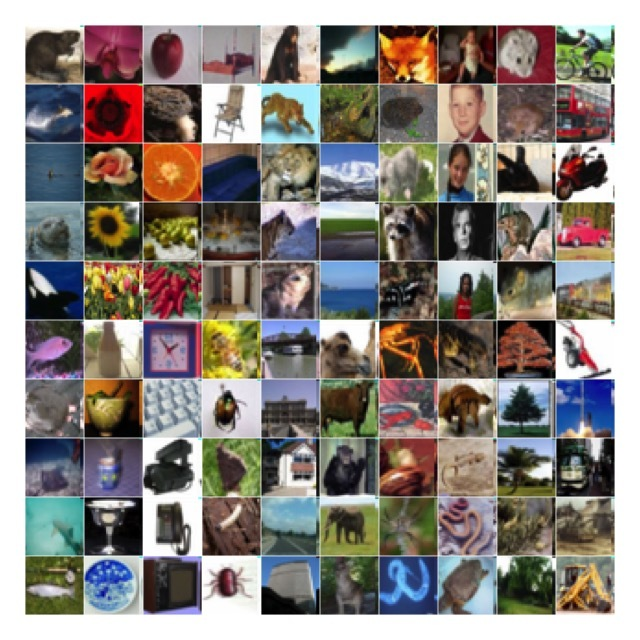
\includegraphics[width=0.5\textwidth]{images/cifar100}
\caption{An example set of images from CIFAR-100. From \cite{cifar100-sample}}
\label{fig:cifar100}
\end{figure}

A particular point of interest with CIFAR-100 is that there are relatively few images per class.
This means that it is a dataset for which overfitting is a critical concern.
Typical algorithms, without any specially designed methods, can often achieve around 60\% accuracy on the testing dataset.
This, however, tends to represent a hard limit, as training accuracy will usually hit nearly 100\% accuracy, meaning that the network has learned all it can from the training dataset.
The difference between testing and training accuracy, especially with the limited data available, is the primary area of improvement for modern algorithms.

We perform a base experiment on a residual network with 30 residual blocks (60 layers), with channel sizes starting at 16 and increasing by a factor of two every 10 layers.
This structure is an adapation of the original residual network, which was built for the ImageNet dataset, to CIFAR-100, which has much smaller images and therefore requires less capacity in the network.
Again utilizing common practice, we use minibatches of size 128, and sample training accuracy every 100 steps.
We allow training to proceed until error rates drop inperceptibly over a reasonably significant period of time; while this requires human judgment, it was also performed due to general time constraints.
We see the expected training accuracy go to 100\%, but the testing accuracy hovers around 65\%, which is also in line with expectations.

In our first experiment, we again use the same basic algorithm first developed for the sine experiment and let the network learn in tenths.
Observing the error rates from the static experiment, we let the network expand every 25 samples (representing 2500 steps).
This is an extremely restrictive network, and our results show that this is perhaps overconstrained for the problem; the training error peaks at 80\% while the testing error hovers around 58\%.
While this is a noticeably poorer result, it is still interesting to note that the generalization appears to be better in this experiment, as the difference between the training and testing error falls from 35\% to 22\%.
Even in the prior static baseline, there was never a comparably small difference between the training and testing error.
This leads us to consider what might be the beginnings of a generalizability metric, which we discuss in the following chapter.

We also note that that accuracy on the dataset is just one measure of precision.
During our experiments, we also log the cross-entropy loss, which provides a sense of not just how likely the network was to get the right answer, but how confidently it did so.
That is, while the accuracy is determined by picking the category with the highest activation, it may have been a very close decision.
For example, on a binary classification problem with classes 0 and 1, where the correct response is nearly always 1, a network with constant output activations $[0.49, 0.51]$ would have extremely low error but high cross-entropy loss.
Using this metric, we note that the cross-entropy loss is lower at the same training error for our methodology, indicating that its outputs are more regularized.

\begin{table}[!htb]
\centering
\caption{CIFAR-100 results}
\label{table:cifar}
\begin{tabular}{@{}lrrr@{}}
\toprule
Network    & Testing Accuracy & Training Accuracy & Training Loss \\ \midrule
Standard   & 0.659            & 0.9927            & 0.0221        \\
Adaptive-1 & 0.582            & 0.8001            & 0.6595        \\
Adaptive-2 & 0.681            & 0.9557            & 0.1379        \\ \bottomrule
\end{tabular}
\end{table}


These results are summarized in table

To improve the performance of this algorithm, we perform another experiment where we gradually allow a limited proportion (50\%) of the network to unfreeze over time.
We believe that this can be helpful in unlocking some of the limited capacity in the network; in particular, we note that the first few convolutional layers are fed into a very narrow pipeline of only 16 filters at full capacity.
Our training algorithm limits this further, which may overly constrict the flow of information through the network.
By leaving at least half of the capacity to be trainable, we attempt to allow sufficient flow for better accuracy.
This hypothesis is borne out by the results, which show that the new network (entitled ``Adaptive-2'' in the figures) is able to demonstrate a small but significant improvement over the standard network.
We achieve a stable testing accuracy of 68\%, but interestingly, our 



\section{Performance}
We note that our algorithm involves nearly no overhead over the original architecture; a simple timing benchmark over 1000 epochs of MNIST indicates a performance difference of 3.5\% (37.9 seconds versus 36.6 seconds), which is well within the margin of error.
Furthermore, by limiting the capacity of the network, we are able to achieve far faster initial training.
The initial timing experiment was performed by applying the algorithm but forcing it to use the full capacity of the network initially; this is far from the original intent.
By utilizing it in the same way as developed for the experiments, the first 1000 epochs of MNIST actually take 11.9 seconds, which is a huge improvement.
This performance boost can make a significant difference over the course of a training cycle.
While the algorithm takes more epochs to converge, the increased speed of working through the initial epochs is a significant boon.
In general, any decrease in performance can likely be attributed to the more intricate methods required to perform basic variable operations, recalling Listing~\ref{lst:var_deconst}.
These are generally considered to be minor; in fact, for most researchers, the choice of deep learning library is rarely for performance reasons, especially for single-GPU servers.
Nearly all of the time spent is within the intricacies of the CUDNN module which interfaces directly with the GPU.
Our algorithm adds effectively no stress to the GPU, and can speed up training even when running at full capacity by fixing portions of the network, thus eliminating the need to perform the expensive gradient calculations.

\chapter{Discussion}
Our results are highly promising, and additionally show some other tendencies, which we highlight in this chapter.
Our algorithm appears to work as a regularizer, ensuring that a network does not devolve into a suboptimal state.
We are also able to see an improvement in generalization compared to standard training regimes, which is a key benefit.
Finally, we list a number of limitations and provide guidance and direction for potential future work.

\section{Regularization}

An important aspect of fixing part of the network capacity is that it prevents the network from diverging significantly.
This is, in effect, a form of regularization, which we can see most clearly in the function regression results.
By fixing the majority of the network, the capability of the network to produce noisy results is far more limited.
This may be an important property even if the network is unable to achieve significant improvements on a dataset, stability is an important goal of any training algorithm.
This stability may also allow the algorithm to perform better, as the moving average becomes less susceptible to noise.
We believe that this virtuous cycle can be further exploited by a more advanced extrapolation of the error curve.
Anecdotal results have indicated that the algorithm does indeed pick more opportune times to expand the network as the fixed capacity increases (and with it, the strength of the regularization), but further work would have be done to verify this effect.

Furthermore, this corroborates the known literature that network capacity is being used inefficiently.
The ability for a network to function well despite only being able to train on a fraction of its capacity indicates a potential overparametrization of the original network.
It would be interesting to apply parameter deletion methods to the frozen capacity, as they generally try to involve minimal perturbation to the network.
This would allow an efficient network to be constructed in-place, without requiring a significant amount of retraining.
We had previously attempted a version of the algorithm that gradually unfreezes the network as an attempt to improve late-stage error, but were unable to detect any major differences between this algorithm and standard training.
This indicates that the retraining process during most parameter deletion methods may be unnecessarily noisy, and we believe that our fixed capacity may help solve this problem.
By utilizing extra capacity to correct for and smooth the errors of the fixed portion, the network is given what is potentially a simpler problem.
We note that this is different from boosting or ensemble architectures due to the high degree of interconnection---as capacity is introduced, it is fully connected to all of the available capacity of the previous and next layers.
This means that the learning is far more organized as a single unit rather than as small substructures.

\section{Generalization}
As we noted briefly in the experiments, one of the interesting trends of the adaptive network was that it tended to overfit less, even if the full results were not as good.
Interestingly, its generalization performance was better than the standard network at the same training error, indicating that it had potentially learned the problem better under a certain metric.
Part of the hope with the algorithm is inspired by the idea that using less parameters prevents overfitting and allows for a model to be more general; this seems to be borne out by the results.
Through various versions of the algorithm, we were able to perform improvements to the testing error consistently; this is despite the standard network having fully utilized the training set, reaching 0\% error.
Our methods have shown consistent improvement, and most interestingly, our final CIFAR-100 test has lower training accuracy but higher testing accuracy than the standard network.

This is an interesting improvement, as the imperfect training accuracy may indicate that further gains could be made on both accuracies, perhaps by better informing the optimizer.
Crucially, the final fully-connected layer's capacity is currently modified along with the last convolutional layer, which could significantly impact the outputs.
In keeping with modern trends that focus on maximizing convolutions throughout the network, residual networks do not depend significantly on fully-connected layers. 
However, we believe that for the purposes of this algorithm, our results demonstrate the potential need for additional capacity that does not change as often.
Along with our good generalization results, performing further higher-level architectural optimizations may help improve results even further. 

\section{Limitations and Future Work}
There are number of topics that were unfortunately outside the realm of reasonable exploration during the course of this thesis.
Many of these pertain to the specifics of our algorithm, which could see significant fine tuning.
While our results are generally good, we believe that that are still major gains to be achieved by continuing along the same directions established by our work.
This thesis provides an interesting result, but also opens up a variety of questions for future investigation.

As noted, whenever possible, we have preferred to maximally utilize the currently available methods rather than performing significant rewrites specific to our problem.
This helped our work maintain its focus on the specifics of improving deep learning training, rather than work on significant reimplementations that would likely introduce new bugs into the system.
At the same time, this could be an area of future work, as we have briefly discussed the potential limitations of using off-the-shelf initializers and optimizers.
These restrictions are generally due to the lack of knowledge within the system, which could significant effects on the training capability of the network.
We noted that our initial sine function approximation network began to learn far slower than expected, which we conjectured to be due to poor initialization.
Furthermore, we were not able to independently verify whether the fixed weights were entirely frozen.
Due to the intracacies of the optimizer, it is possible that momentum terms, or just other modifications from standard gradient descent led our network to keep changing even when it was fixed.
We expect that Tensorflow's ability to stop gradients from flowing through the fixed sections should have effectively done the job, but it may have taken a few more epochs.
In order to solve these issues, we would have to perform custom implementations of Adam, Xavier, and perhaps other components as well that are aware of the capacity limitations we impose.
This would likely complicate the codebase significantly, as Tensorflow operations are not as easy to develop.
Some algorithmic questions also remain, such as the correct initialization values for added capacity.
These would involve significant new testing and theory to determine.

We also believe that sparsity is an interesting topic but were unable to cover it within this thesis.
In his work on spatially-sparse convolutional neural networks \cite{graham2014spatially}, Graham noted that there are potential improvements in architecture by performing sparse convolutions.
Tensorflow does not support such functionality at the moment, although it appears that they may be planning its development for the future \cite{spatiallysparseconv}.
For our experiments, we continue to rely on densely-connected convolutional layers.
Apart from the natural computational efficiency, we note that sparse networks are generally utilized in problems where the problem is seen as less compact or able to exploit the sparse connections---such is not often the case for image classification, which is our primary subject in this thesis.
We do note, however, that this would be a very interesting way of implementing dynamic network capacity that extends beyond our current implementation.
Importantly, this may allow the network to suffer less shock as additional capacity is added by initially minimizing the number of connections between the original or fixed section and the newly-added training section.
In this way, the sections can be trained somewhat like an ensemble of networks that gradually begins to learn some capacity for communication.
Therefore, controlling this dynamic would be an extremely powerful tool.

Another area of interest is the amount of dynamicism in the network architecture.
Srivastava et al. explore Highway Networks \cite{srivastava2015highway}, which allow learned connections to form between any two layers.
This is obviously a far more complex architecture, requiring additional connections in the network, but may be thought of as a higher-level abstraction over residual networks.
Allowing the network to develop not just in per-layer capacity but also in layer connections could allow better mutability.
The results regarding the training accuracy have shown that fixing significant capacity limits the ability of the network to overcome some of the errors caused by limitations of capacity.
However, it is possible that increased connections between each layer would provide the necessary adaptations to learn the problem well, without adding a significant number of parameters to the whole network.

While the hyperparameters for our algorithm were generally chosen on inspection of the testing baseline, we note that it may be possible to develop a reasonable set of defaults for an average user.
This would be highly beneficial, as it further removes the necessity of tuning.
Apart from edge cases which would be known to the user, it seems that basic analysis can indicate when convergence is beginning, and the algorithm can adjust accordingly.
A improved algorithm would perhaps entail a more detailed analysis of previous errors beyond a simple moving average, which would allow it to be smarter about when a resize is necessary, as opposed to occasionally falling for noise in the error.
Many small tweaks could be developed as a result of more extensive testing of the algorithm to better understand its behavior on a wider range of learning problems.

Another direction we see is in the potential for live user intervention during training.
In general, most modern methods do not allow any changes to the architecture, meaning that if certain parameters are set poorly but go unnoticed, significant time can be lost as the network will have to start training from scratch.
Technically, this functionality is available in a very crude sense in our current software, as the data is mostly saved into checkpoints that could be loaded and overwritten.
This means that by overwriting the current state variables of the algorithm, subsequent runs would then adopt the updated values.
Especially with Google's Tensorboard software, which allows a Tensorflow network to show its computational graph, log various properties, and much more, we see the potential for users to gradually tune a network on-the-fly.
In conjunction with our algorithm providing suggestions on network changes, it would be interesting to allow a more technical user to query specific statistics about the network, then make decisions on tuning without necessitating a new and costly training cycle.
This kind of fine-grained architectural control during runtime is completely new to the literature, so we see our work as a foundational first step.

\chapter{Conclusion}
\section{a brief summary of results}
\emph{ < what the section title says > }

\section{Future Work and Further Notes}

\emph{ < talk about shortcut connections, different trainable parameters, also extend literature to other directions of optimization > }


\nocite{*}
\bibliographystyle{acm}
\bibliography{ref}

\begin{center}
\emph{This work represents }
\end{center}
\end{document}